% -*- coding: UTF-8 -*-
% hurlex-chapt12.tex
% hurlex 开发文档 第12章内容

\section {内核线程的创建与切换}

\par 这一章我们将讨论内核线程的创建与切换。

\par 首先给出内核线程的含义,此处的内核线程作为运行在内核态的一个逻辑执行流,拥有私有的栈空间。但是除了这个私有的栈之外,\allowbreak
不拥有其它的资源。所有的内核线程拥有相同的页表,共享所有的全局数据。

\par Intel的x86CPU提供任务切换机制是使用TSS段进行切换,这么做比较繁琐且效率较低,现代的OS都不会完全采用硬件切换机制。本章所\allowbreak
阐述的任务切换只发生在内核态,不涉及特权级的转移过程,所以可以完全由硬件实现。而且这种实现用在用户级的线程库中亦可,大家有兴趣\allowbreak
的话可以仿照这个思路实现用户级线程库。

\par 任务的切换必然涉及到现场的保护与恢复,所以就必然需要一个数据结构来保存这些现场信息。这个数据结构中一般也会放置任务相关的\allowbreak
一些信息并且以链表之类的方式组织起来,这个结构被称之为PCB(Process Control Block)或者TCB(Task Control Block)。相关定义如下:

\begin{lstlisting}[language = C, caption = include/task.h]
#ifndef INCLUDE_TASK_H_
#define INCLUDE_TASK_H_

#include "types.h"
#include "pmm.h"
#include "vmm.h"

// 进程状态描述
typedef
enum task_state {
	TASK_UNINIT = 0, 	// 未初始化
	TASK_SLEEPING = 1, 	// 睡眠中
	TASK_RUNNABLE = 2, 	// 可运行(也许正在运行)
	TASK_ZOMBIE = 3, 	// 僵尸状态
} task_state;

// 内核线程的上下文切换保存的信息
struct context {
	uint32_t esp;
	uint32_t ebp;
	uint32_t ebx;
	uint32_t esi;
	uint32_t edi;
	uint32_t eflags;
};

// 进程内存地址结构
struct mm_struct {
	pgd_t *pgd_dir; 	// 进程页表
};

// 进程控制块 PCB 
struct task_struct {
	volatile task_state state; 	// 进程当前状态
	pid_t 	 pid; 			// 进程标识符
	void  	*stack; 		// 进程的内核栈地址
	struct mm_struct *mm; 		// 当前进程的内存地址映像
	struct context context; 	// 进程切换需要的上下文信息
	struct task_struct *next; 	// 链表指针
};

// 全局 pid 值
extern pid_t now_pid;

// 内核线程创建
int32_t kernel_thread(int (*fn)(void *), void *arg);

// 线程退出函数
void kthread_exit();

#endif 	// INCLUDE_TASK_H_
\end{lstlisting}

\par 除了描述每一个任务信息的结构,还需要将这些结构组织起来并且引入调度机制。相关的头文件和定义如下:

\begin{lstlisting}[language = C, caption = include/sched.h]
#ifndef INCLUDE_SCHEDULER_H_
#define INCLUDE_SCHEDULER_H_

#include "task.h"

// 可调度进程链表
extern struct task_struct *running_proc_head;

// 等待进程链表
extern struct task_struct *wait_proc_head;

// 当前运行的任务
extern struct task_struct *current;

// 初始化任务调度
void init_sched();

// 任务调度
void schedule();

// 任务切换准备
void change_task_to(struct task_struct *next);

// 任务切换
void switch_to(struct context *prev, struct context *next);

#endif 	// INCLUDE_SCHEDULER_H_
\end{lstlisting}

\par 本章不会采用复杂的调度策略,操作系统理论中各种调度算法都不会在这里实现。本章主要目的是说明白任务切换的原理。所以任务\allowbreak
组织的方式就是一个单向循环链表,调度程序每次选择当前任务的下一个任务运行。如果你有兴趣,可以自己实现更好的调度算法。大家完全\allowbreak
可以在PCB里增加新的数据成员,实现带有优先级的任务切换机制。

\par 在进行任务切换之前,内核原先的执行流还没有一个结构来保存其信息,所以需要在初始化调度之前给原始的执行流创建PCB信息。\allowbreak
这里模仿Linux内核早期的做法,将PCB放置在线程栈的最低处。初始化的代码如下:

\begin{lstlisting}[language = C, caption = kernel/sched/sched.c]
#include "sched.h"
#include "heap.h"
#include "debug.h"

// 可调度进程链表
struct task_struct *running_proc_head = NULL;

// 等待进程链表
struct task_struct *wait_proc_head = NULL;

// 当前运行的任务
struct task_struct *current = NULL;

void init_sched()
{
	// 为当前执行流创建信息结构体 该结构位于当前执行流的栈最低端
	current = (struct task_struct *)(kern_stack_top - STACK_SIZE);

	current->state = TASK_RUNNABLE;
	current->pid = now_pid++;
	current->stack = current; 	// 该成员指向栈低地址
	current->mm = NULL; 		// 内核线程不需要该成员

	// 单向循环链表
	current->next = current;

	running_proc_head = current;
}
\end{lstlisting}

\par 调度函数很容易理解,每次都返回当前任务的下一个任务。代码如下:
\footnote{这里的调度函数留给大家自由发挥,去自由实现各种高端的调度算法。}

\begin{lstlisting}[language = C, caption = include/sched.h]
void schedule()
{
	if (current) {
		change_task_to(current->next);
	}
}

void change_task_to(struct task_struct *next)
{
	if (current != next) {
		struct task_struct *prev = current;
		current = next;
		switch_to(&(prev->context), &(current->context));
	}
}
\end{lstlisting}

\par 具体的切换操作由汇编实现,分别是保存当前任务的执行上下文和切换到下一个任务去。代码如下:

\begin{lstlisting}[language = {[x86masm]Assembler}, caption = kernel/sched/switch\_to.s]
[global switch_to]

; 具体的线程切换操作,重点在于寄存器的保存与恢复
switch_to:
        mov eax, [esp+4]

        mov [eax+0],  esp
        mov [eax+4],  ebp
        mov [eax+8],  ebx
        mov [eax+12], esi
        mov [eax+16], edi
        pushf
        pop ecx
        mov [eax+20], ecx

        mov eax, [esp+8]

        mov esp, [eax+0]
        mov ebp, [eax+4]
        mov ebx, [eax+8]
        mov esi, [eax+12]
        mov edi, [eax+16]
        mov eax, [eax+20]
        push eax
        popf
 	
        ret
\end{lstlisting}

\par 经过上面的铺垫,重头戏就是接下来的切换了。内核线程的创建和退出函数的实现如下:

\begin{lstlisting}[language = C, caption = include/task.h]
#include "gdt.h"
#include "pmm.h"
#include "vmm.h"
#include "heap.h"
#include "task.h"
#include "sched.h"
#include "string.h"
#include "debug.h"

// 全局 pid 值
pid_t now_pid = 0;

// 内核线程创建
int32_t kernel_thread(int (*fn)(void *), void *arg)
{
	struct task_struct *new_task = (struct task_struct *)kmalloc(STACK_SIZE);
	assert(new_task != NULL, "kern_thread: kmalloc error");

	// 将栈低端结构信息初始化为 0 
	bzero(new_task, sizeof(struct task_struct));

	new_task->state = TASK_RUNNABLE;
	new_task->stack = current;
	new_task->pid = now_pid++;
	new_task->mm = NULL;

	uint32_t *stack_top = (uint32_t *)((uint32_t)new_task + STACK_SIZE);

	*(--stack_top) = (uint32_t)arg;
	*(--stack_top) = (uint32_t)kthread_exit;
	*(--stack_top) = (uint32_t)fn;

	new_task->context.esp = (uint32_t)new_task + STACK_SIZE - sizeof(uint32_t) * 3;

	// 设置新任务的标志寄存器未屏蔽中断,很重要
	new_task->context.eflags = 0x200;
	new_task->next = running_proc_head;
	
	// 找到当前进任务队列,插入到末尾
	struct task_struct *tail = running_proc_head;
	assert(tail != NULL, "Must init sched!");

	while (tail->next != running_proc_head) {
		tail = tail->next;
	}
	tail->next = new_task;

	return new_task->pid;
}

void kthread_exit()
{
	register uint32_t val asm ("eax");

	printk("Thread exited with value %d\n", val);

	while (1);
}

\end{lstlisting}

\par 内核退出函数在这里只实现了简陋的一部分,标准做法是将退出线程的PCB结构转移到不可调度链表去,等待其他线程join后再\allowbreak
清理结构。这个留给大家自由实现吧,可以自由发散思维去做。

\par 这里的内核线程的创建和切换过程可能有些晦涩,其切换的重点在于switch\_to函数最后的ret指令。在ret指令返回之前,由于之前的\allowbreak
执行现场已经被切换,特别是esp指针指向的栈被切换了,所以ret指令弹出的返回地址自然就变成了另一个执行流之前调用任务切换函数\allowbreak
之前保存的返回地址了。kernel\_thread函数便是通过构造出这样一个切换后可以弹出执行地址的初始栈来实现的。
\footnote{如果理解起来依旧有困难的话不妨在纸上画画调用栈,这样比较好理解。}

\par 解决了所有切换的问题之后,剩下的只是时间片的问题了。可能大家已经想到了,这个调度函数最终是要由timer中断函数来执行的。\allowbreak
我们修改timer中断的处理函数如下:

\begin{lstlisting}[language = C, caption = drivers/timer.c]
void timer_callback(pt_regs *regs)
{
	schedule();
}
\end{lstlisting}

\par 在定时器初始化之后,我们开启INTR中断。此时timer中断会按照之前设定好的工作频率来执行调度任务。

\par 我们在初始化函数里测试下,代码如下:

\begin{lstlisting}[language = C, caption = init/entry.c]

... ...

int flag = 0;

int thread(void *arg)
{
	while (1) {
		if (flag == 1) {
			printk_color(rc_black, rc_green, "B");
			flag = 0;
		}
	}

	return 0;
}

void kern_init()
{
	init_debug();
	init_gdt();
	init_idt();

	console_clear();
	printk_color(rc_black, rc_green, "Hello, OS kernel!\n\n");

	init_timer(200);

	printk("kernel in memory start: 0x%08X\n", kern_start);
	printk("kernel in memory end:   0x%08X\n", kern_end);
	printk("kernel in memory used:   %d KB\n\n", (kern_end - kern_start) / 1024);
	
	// show_memory_map();
	init_pmm();
	init_vmm();
	init_heap();

	printk_color(rc_black, rc_red, "\nThe Count of Physical Memory Page is: %u\n\n", phy_page_count);
	test_heap();

	init_sched();

	kernel_thread(thread, NULL);

	// 开启中断
	enable_intr();

	while (1) {
		if (flag == 0) {
			printk_color(rc_black, rc_red, "A");
			flag = 1;
		}
	}

	while (1) {
		asm volatile ("hlt");
	}
}
\end{lstlisting}

\par 编译运行后,我们看到了完美交替输出的A和B,如图所示:

\begin{figure}[ht]
      \centering
      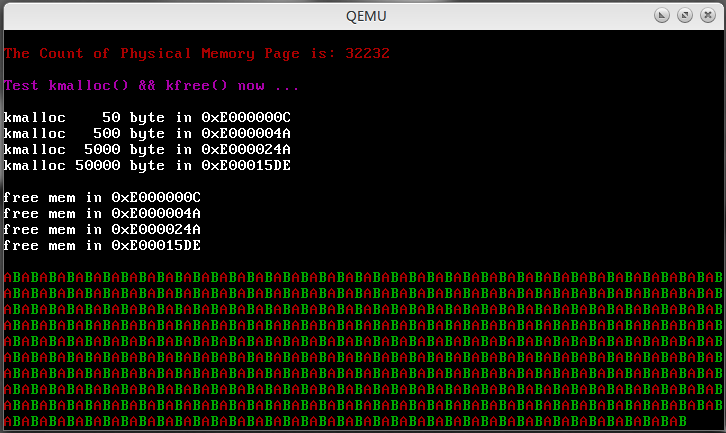
\includegraphics[scale=0.6]{picture/chapt12/KTHREAD.png}
      \caption{测试内核线程切换}
\end{figure}

